\documentclass[a4paper,12pt]{article}
\usepackage{hyperref}
\usepackage{graphicx}
\usepackage{geometry}
\usepackage{times}
\usepackage{amsmath}
\usepackage{amssymb}
\usepackage{enumitem}

\def\name{Benjamin Pope}

\setlength\parindent{2em}
\setlist[description]{leftmargin=\parindent,labelindent=\parindent}
\begin{document}

\title{Using a Doubly-Diffractive Pupil to set the Wavelength Scale for TOLIMAN
}
\author{Benjamin Pope}
%{\huge Curriculum Vitae -  \name}
\textwidth=19.0cm
\textheight=22.5cm
\abovedisplayskip=0pt
\belowdisplayskip=0pt
\maketitle

\section{Rationale}

The goal of the TOLIMAN mission is to measure the angular separation of the stars $\alpha$~Cen~A and~B to a precision of better than $\sim 0.5 \mu$as. We cannot do this straightforwardly: the telescope is not perfectly rigid, and we get optical distortions and changes in focus which mean that the plate scale $p$ changes and the separation of the stars on the detector is not fixed.

The idea of a diffractive pupil in TOLIMAN is that we can use a very complicated diffraction pattern which is known independently of the plate scale and any distortions. By imprinting this pattern in the very first pupil plane we ensure that it depends on all aberrations in the system, and we can ``count fringes'' to get good astrometry.

It is clear that in either of the limits $\Delta p \rightarrow 0$ or $\Delta \lambda \rightarrow 0$, we can do simple pixel counting or fringe counting respectively and any uncertainty in the other variable is irrelevant. But the PSF on the detector is some (complicated) function 

\begin{equation}
f(p\lambda\cdot(\text{pix}-\text{pos}))
\end{equation}

such that if $p$ and $\lambda$ vary oppositely and in proportion, the PSF looks the same on our detector but the stars appear to change in separation in both fringe and pixel counts. Whichever has a lower noise floor can be used to calibrate the other; I therefore suspect that we really only need to get one of these to the $10^-6$ level of precision.

In order for TOLIMAN to work, we need to fix at least one of $\dfrac{\Delta \lambda}{\lambda}$ or $\dfrac{\Delta p}{p}$ to better than $10^{-6}$ or so. But we not only expect focal length (and therefore plate scale) changes from the satellite's thermal variations, but also changes in the stellar spectrum and therefore the effective wavelength due to intrinsic stellar variability. 

(I think, but am not completely sure, that the effective wavelength, and perhaps a few low order moments of the spectrum, are all I think we should really need: a speckle at $n \lambda/D$ is only sensitive to spectral features at $R\lesssim n$, so given a 4~arcsec binary separation and a 400~$\mu$as $\lambda/D$, we only go up to $n =$ a few tens in the relevant part of our field of view).

\section{Intrinsic Stability}

First we want to investigate how significant stellar variability actually is in affecting our wavelength scale. While $\alpha$~Cen is a well-observed system, publicly-available spectra are geared towards extracting radial velocities or lineshapes, and have calibration lines imposed and systematics in the continuum on a length scale of $\sim$~tens of nm. I therefore used \texttt{pysynphot} and the \textsc{phoenix} stellar model grids to simulate a star with the same parameters as each of the $\alpha$~Cen stars.

Following Nem Jovanovic, I then considered what happens if you allow the surface to be covered in spots with coverage between $0 -- 15\%$, with a temperature of 4700~K. This is not very rigorous but is a quick stab. I then selected a bandpass 

\begin{equation}
b \propto \exp{ ((\dfrac{x-x_0}{2\sigma})^8)},
\end{equation}

a super-Gaussian with a very flat top smoothly rolling to steep sides, and reported the fractional change in centre wavelength between 0\% and 15\% -- spotted stars at each band centre and bandwidth. Stability curves are displayed in Figure~\ref{stability}, with the key result being that narrow bands can be chosen to be passively stable at the $10^{-6}$ level, but not broad bands. This is a potential solution to our problem: find a highly stable bandpass and choose a band around that -- but in doing this we lose a lot of throughput. Perhaps there is a better way.

\begin{figure}
\centering
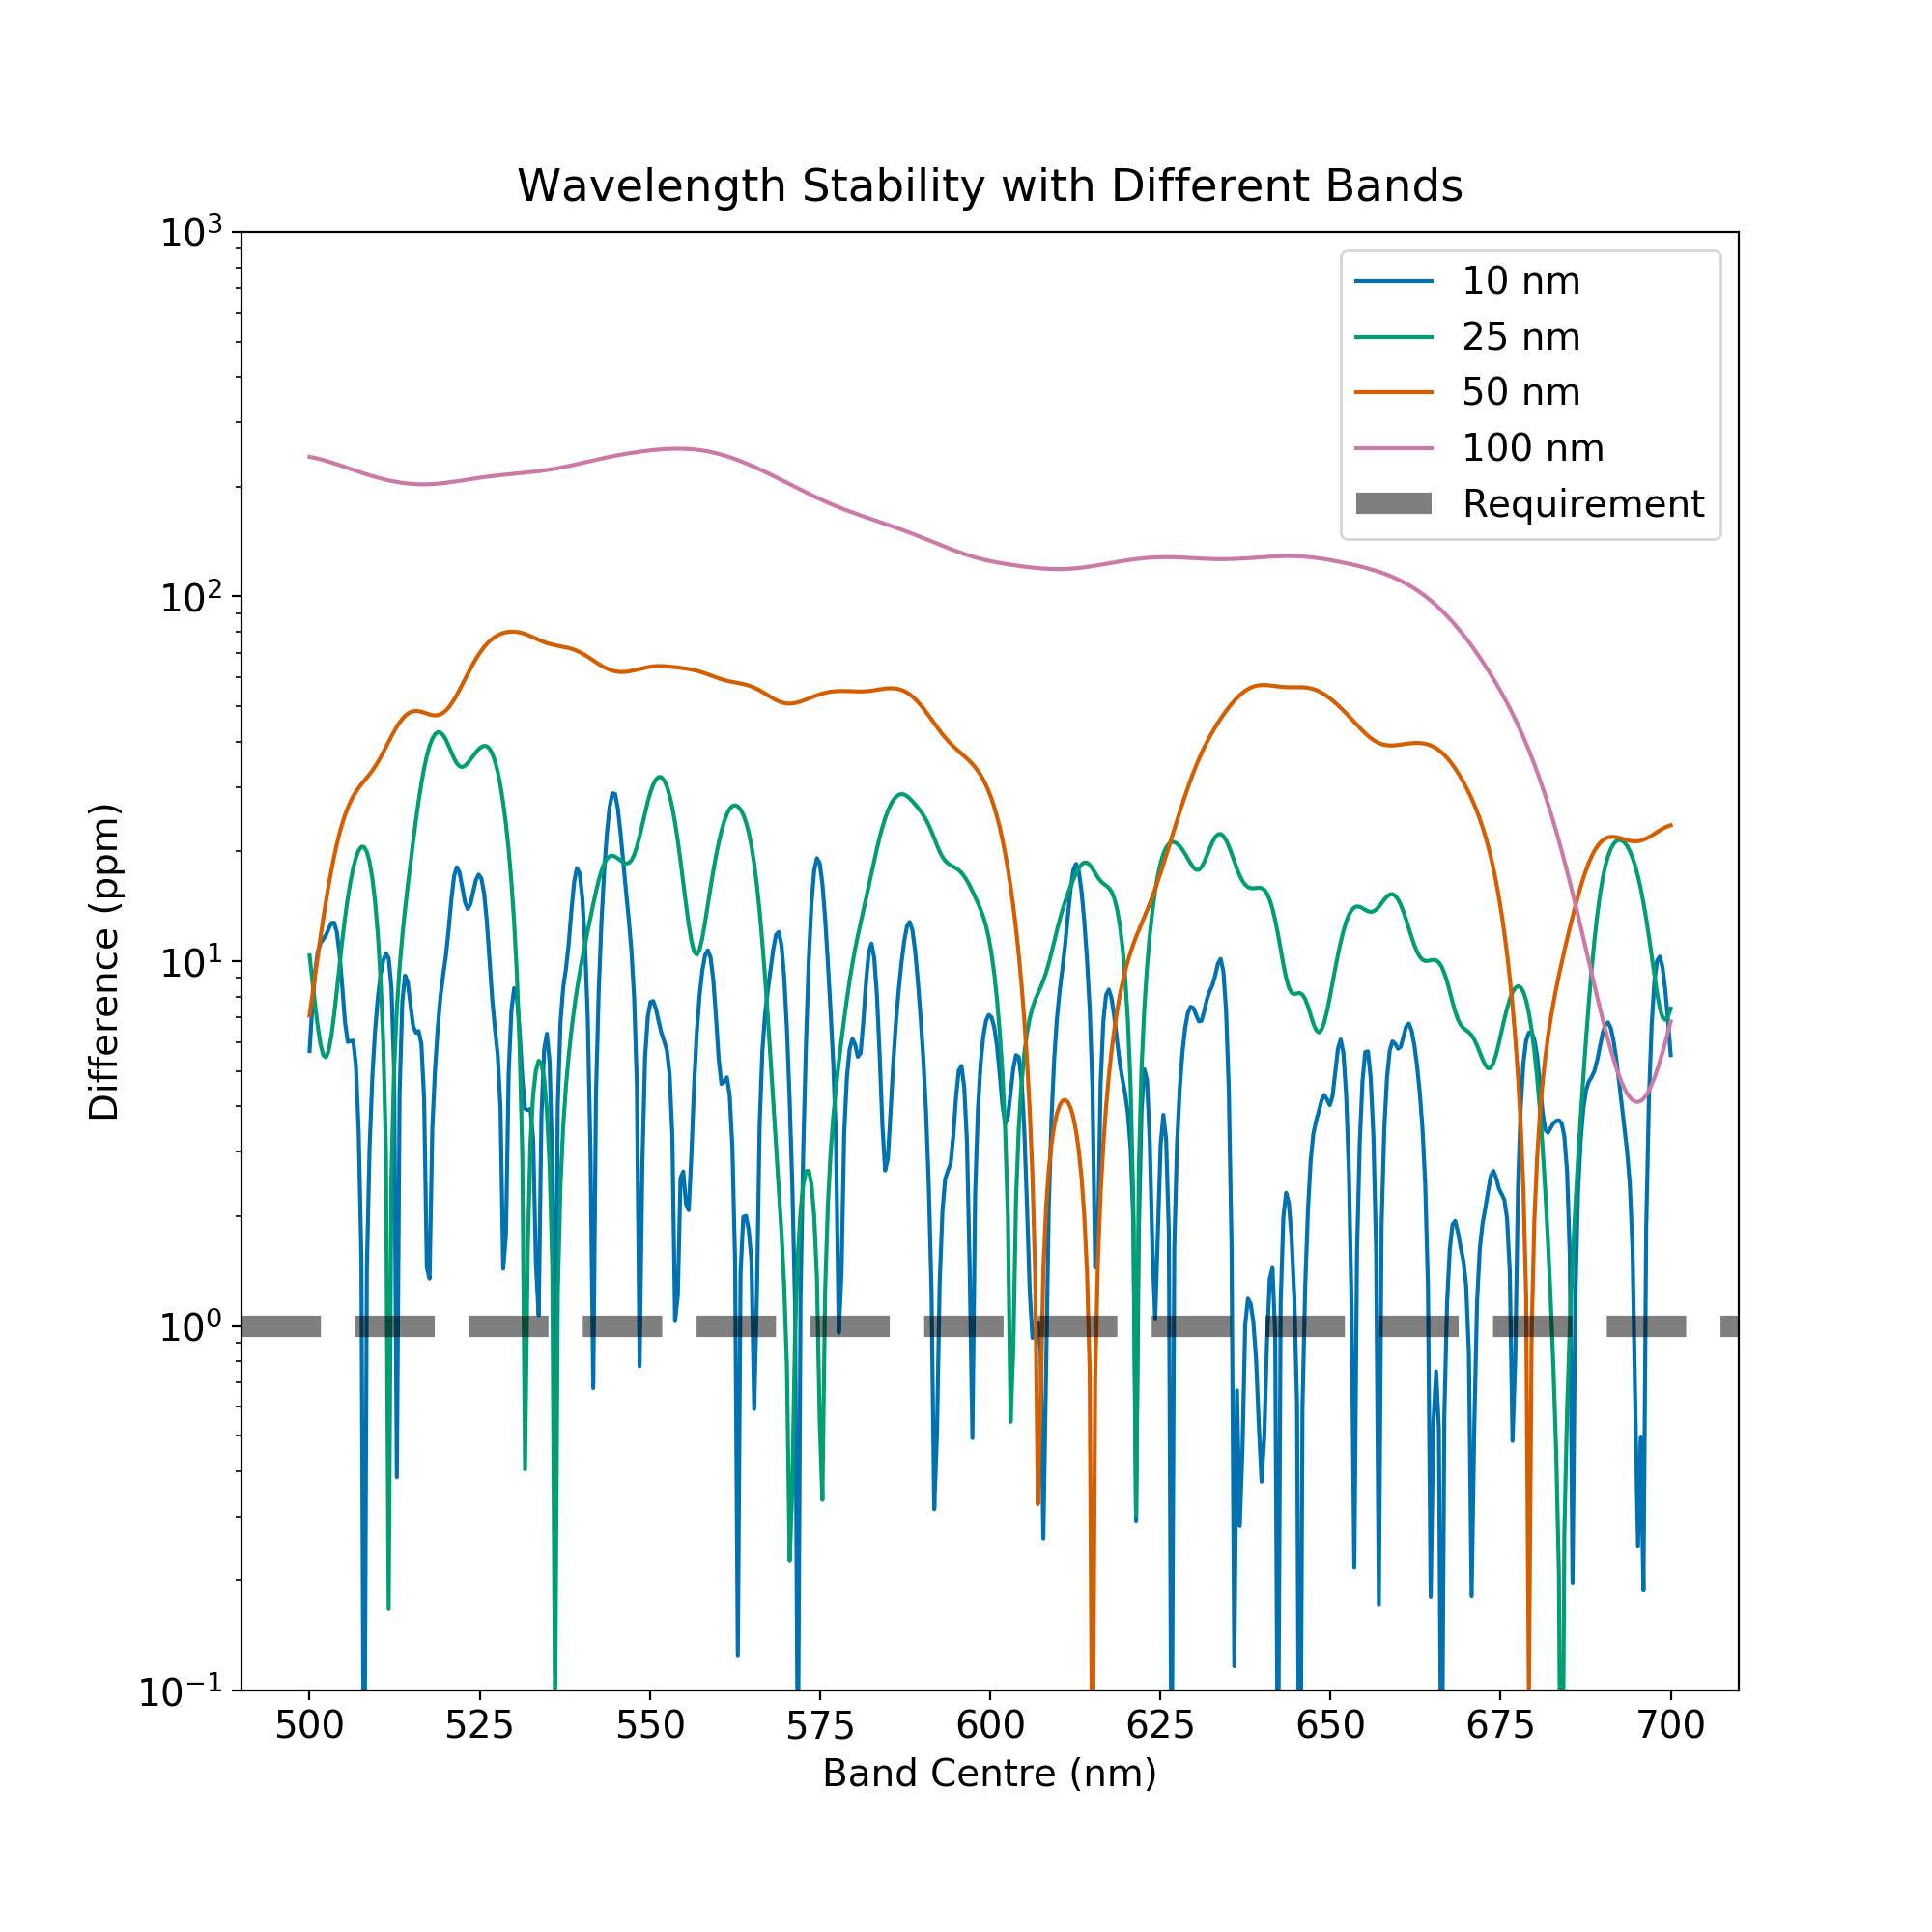
\includegraphics[width=0.75\textwidth]{bands.png}
\caption{Passive wavelength stability as a function of band centre, for bandwidths from 10~nm to 100~nm.}
\label{stability}
\end{figure}

\section{Stellar Spectral Features}

If the stellar variability is one of our key problems, the stellar spectrum nevertheless offers a solution. Both stars have spectra imprinted with deep (tens of percent), narrow ($\sim$~nm) spectral lines every few nm across much of the visible band. We can use these to get an absolute wavelength calibration regardless of plate scale. I considered two possibilities: using the primary PSF's wavelength dependence, or using a secondary diffraction spot. As we shall see, the former appears infeasible, but the latter approach seems promising.

\subsection{Zeroth-Order PSF Modelling}

I calculated an ensemble of PSFs with wavelength across 600-700~nm across a 10 arcsec field of view with a 50 nm plate scale - being extremely generous - and used PCA to find out the underlying dimensionality of this space. This is the approach taken in multimode fibre spectroscopy and we would expect a space of dimension $N$ to get $N$ channels across our bandpass. The fraction of variance explained by each principal component is a proxy for whether it senses anything, and as we see in Figure~\ref{zeroth}, this decreases steadily to a floor at 20-30. Visual inspection of the components shows the first couple of dozen look physical and the remainder are noisy. I therefore say we can probably get at most $(100~\text{nm})/20 = 5~\text{nm}$ resolution by this method, which would seem insufficient to grab any spectral lines. 


\begin{figure}
\centering
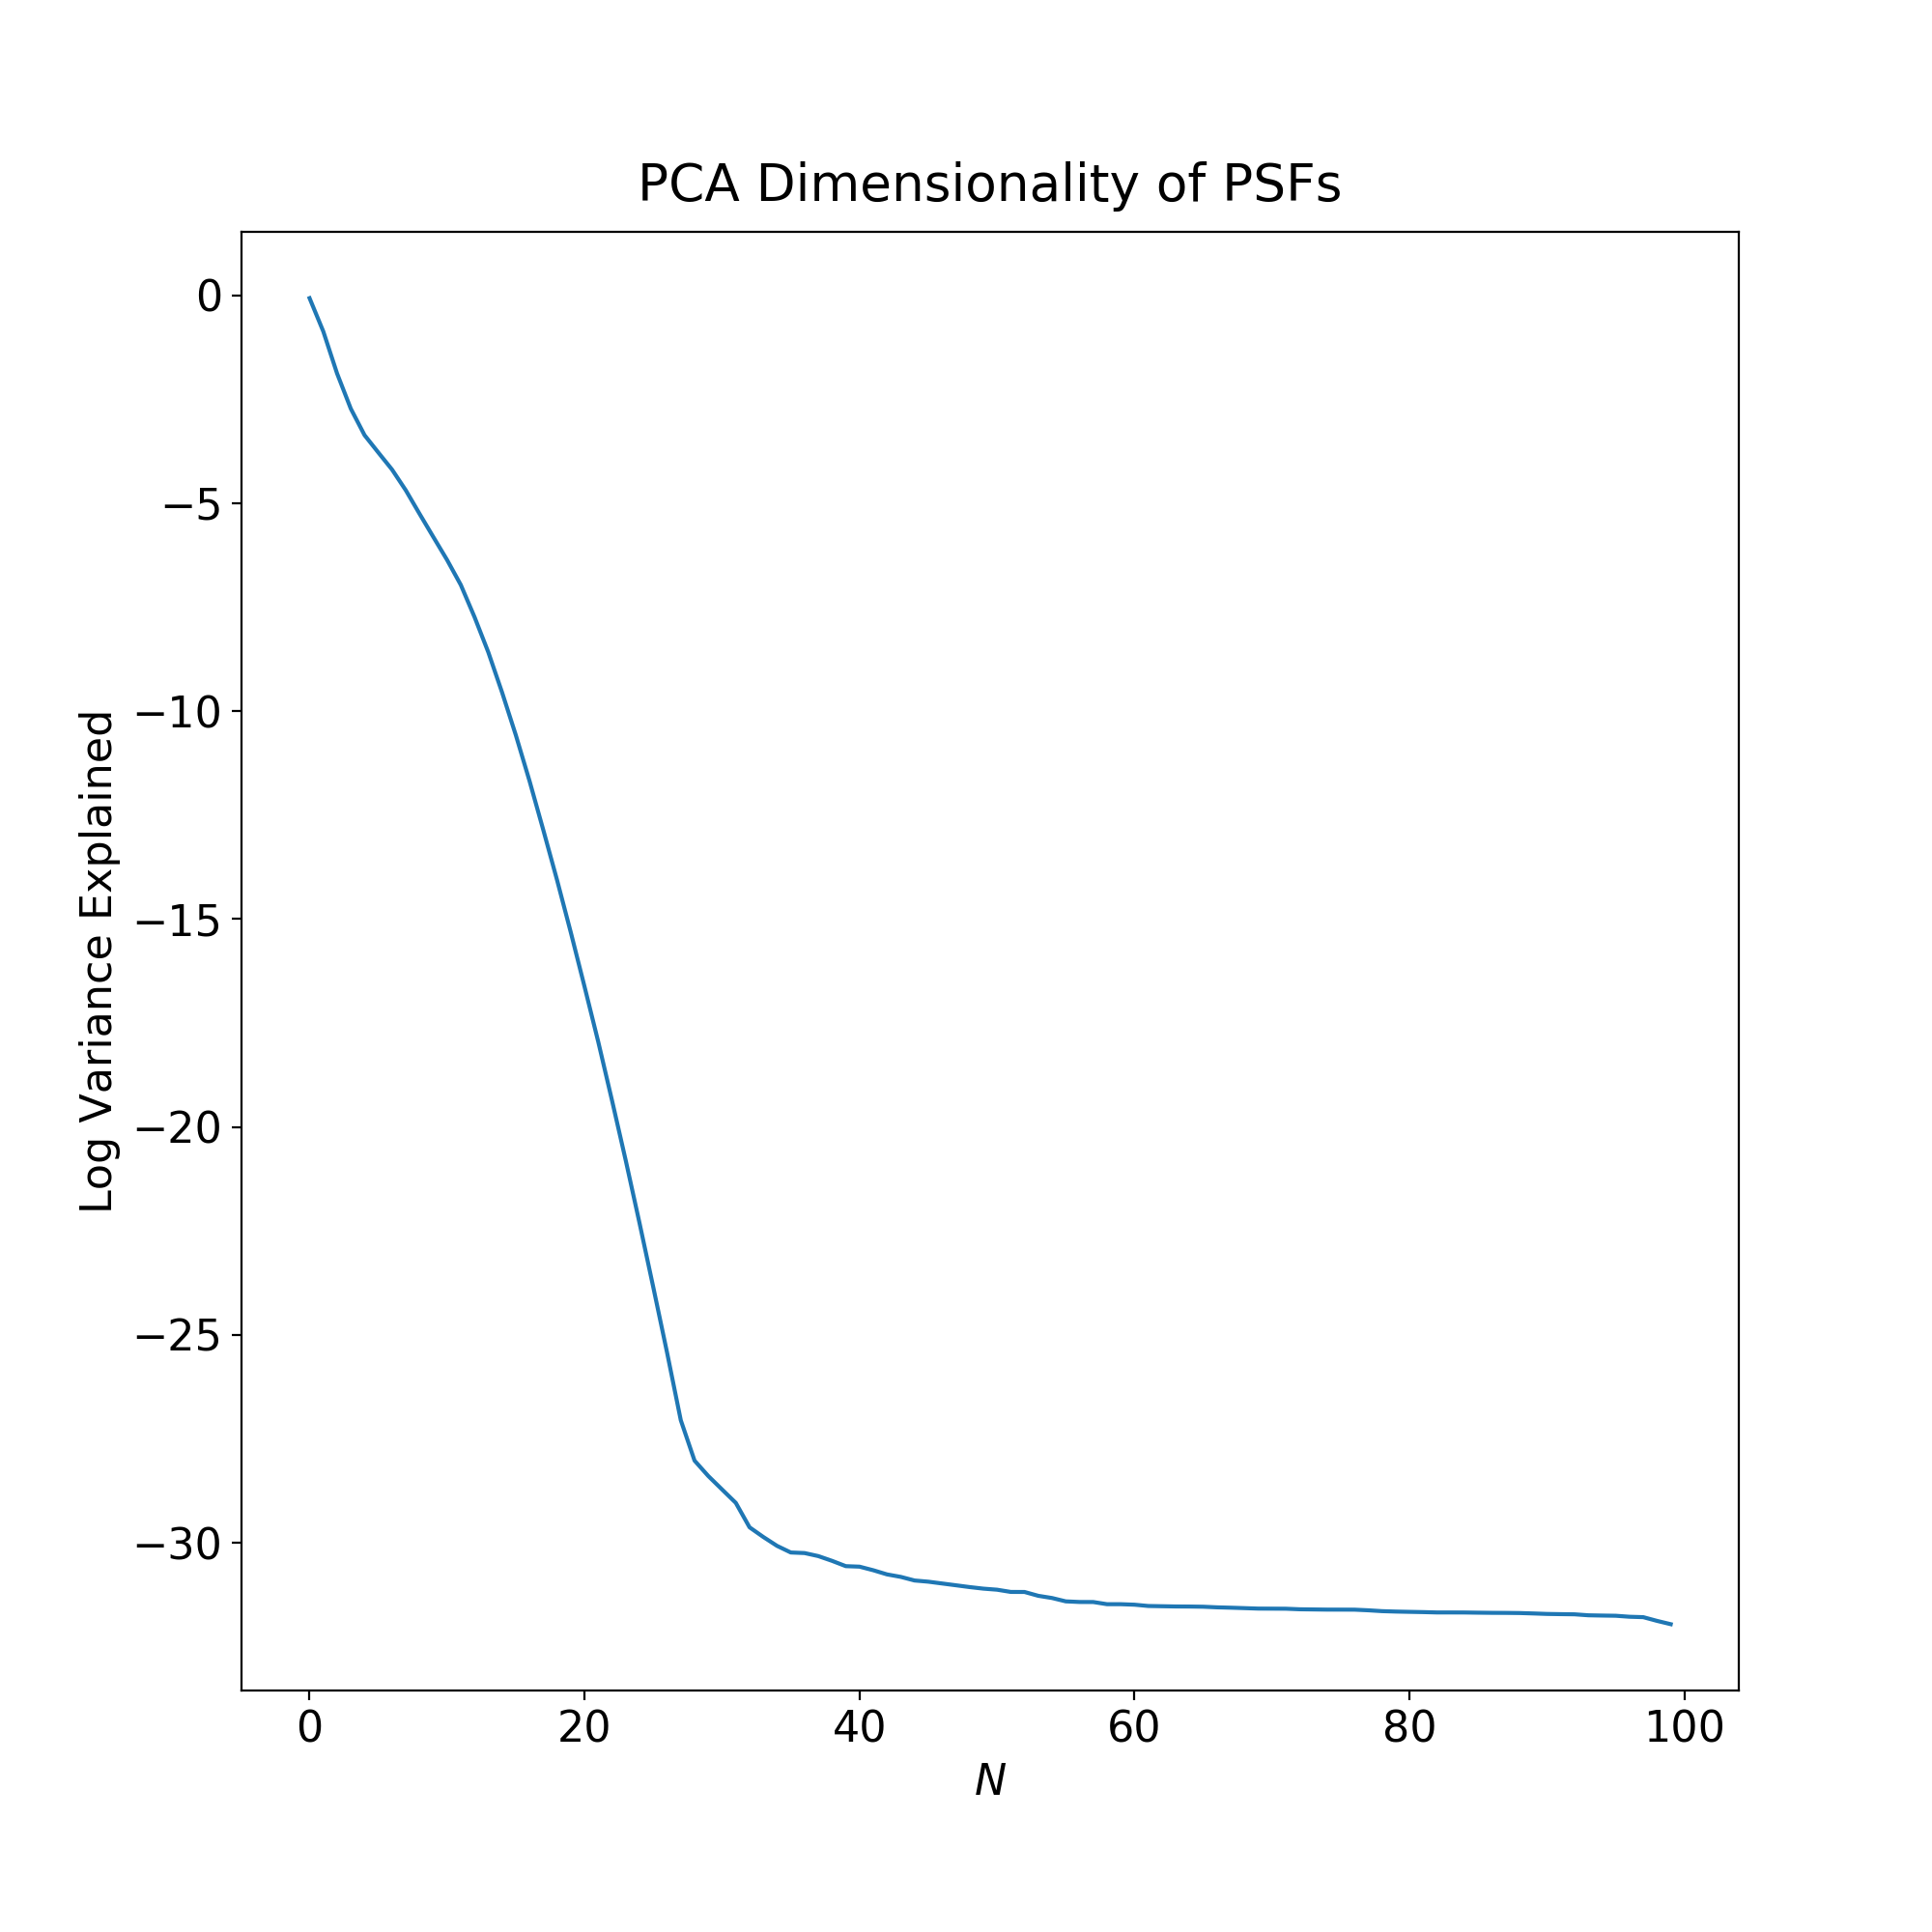
\includegraphics[width=0.75\textwidth]{dimension.png}
\caption{The fraction of variance explained by each principal component falls rapidly to a floor at about 20. I therefore assert that at most we get about 20-30 channels across our bandpass.}
\label{zeroth}
\end{figure}

\subsection{First Order Diffraction}

What if we use a doubly-diffractive pupil, to send a PSF copy out to large angles? We can get a much higher spectral resolution this way. Recall that the familiar grating equation for resolving power $R = mN$ is derived from the width of the sinc-function core of a grating windowed to N lines, operating at $m$th order. A similar analysis says that if the PSF core has width $\Delta \theta$ and we diffract the centre wavelength to an angular distance $\kappa$, then $R = \dfrac{\kappa}{\Delta \theta}$. If we send it to $\sim$ an arcminute, with a $\Delta\theta \sim \lambda/D = 400\text{mas}$, we have a resolving power of several hundred and this approach is feasible.

I did a simple simulation to investigate this. I generated a diffraction pattern at 900 pixels from centre with a plate scale of 0.1~arcsec, shown in Figure~\ref{firstorder}, consisting of 300 PSFs at each wavelength from 6125 to 6875 angstroms. I added these together, weighted by a spectrum shown in Figure~\ref{spectrum}. I then simply used \texttt{scipy.optimize.minimize} to fit this with a linear combination of the input PSFs, constraining their weights to be in $[0,1]$, and achieved a remarkably good fit with even such a simple algorithm. The centroids of the input and recovered spectrum differ by 18~ppm, which is just a little above the noise floor we want, but I suspect this can be improved with better algorithms, and we certainly see the spectral features very clearly.

\begin{figure}
\centering
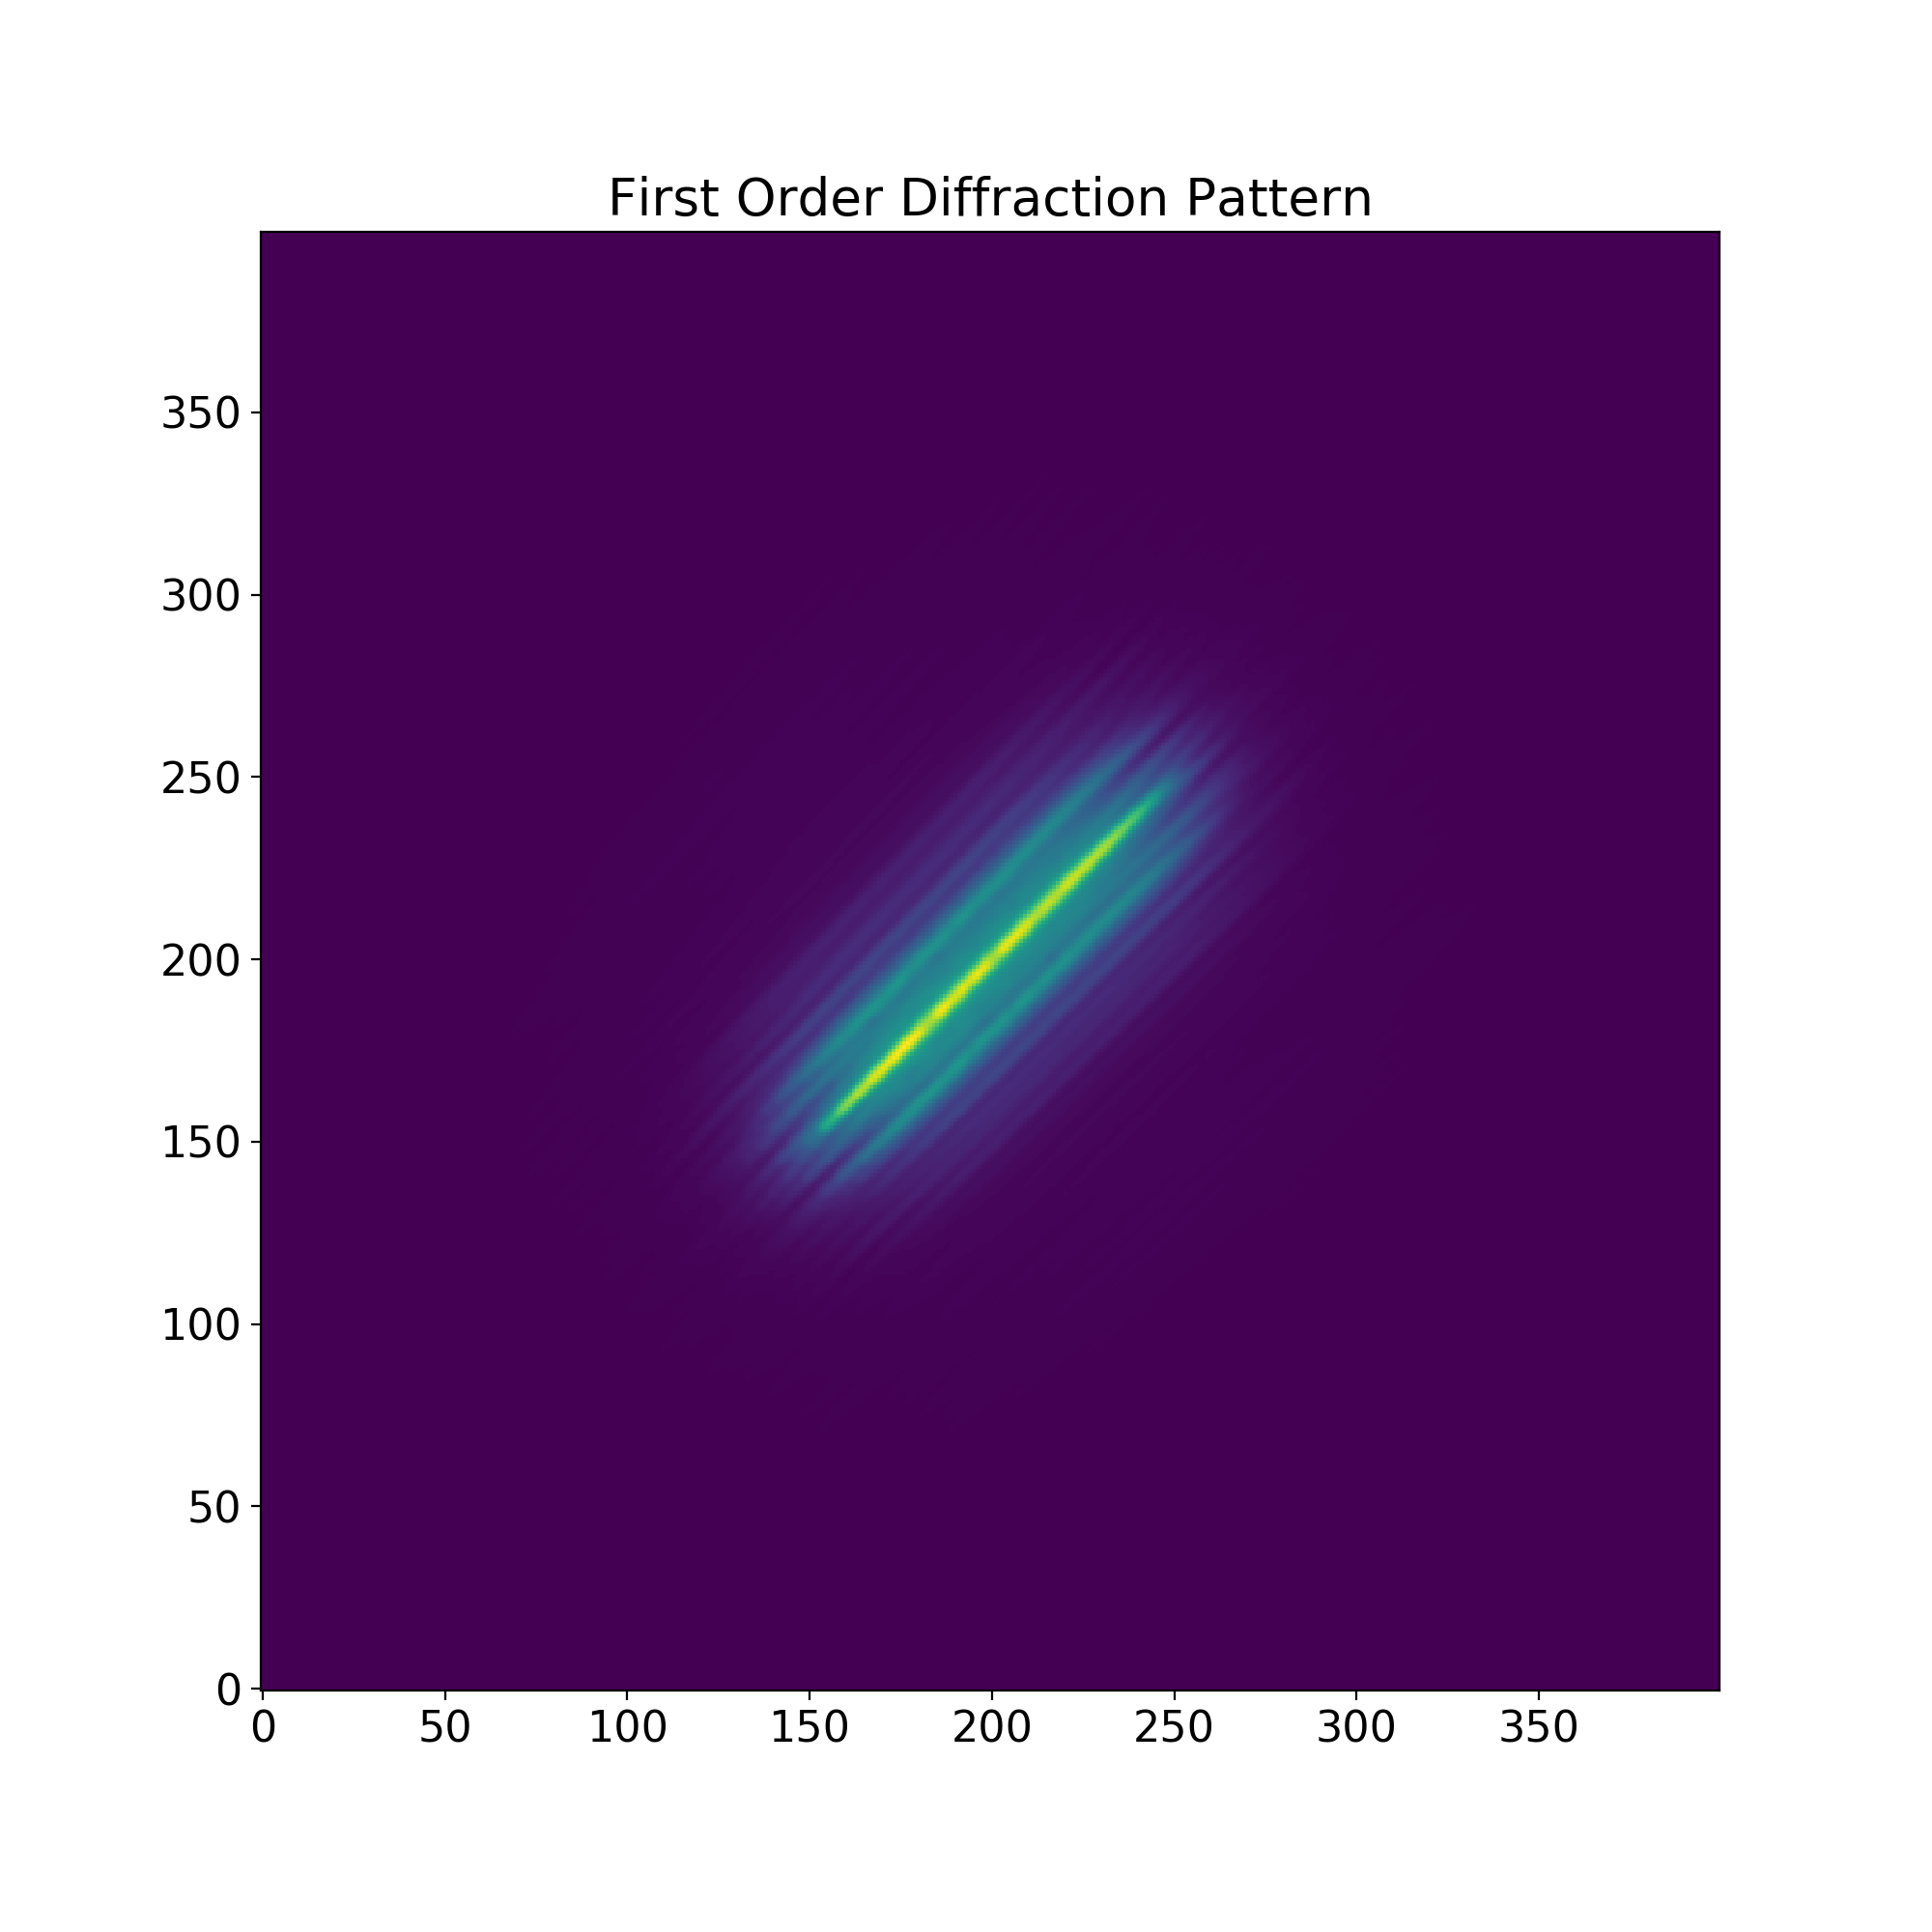
\includegraphics[width=0.75\textwidth]{firstorder.png}
\caption{First order diffraction pattern, imprinted with the spectrum shown in Figure~\ref{spectrum}.}
\label{firstorder}
\end{figure}

\begin{figure}
\centering
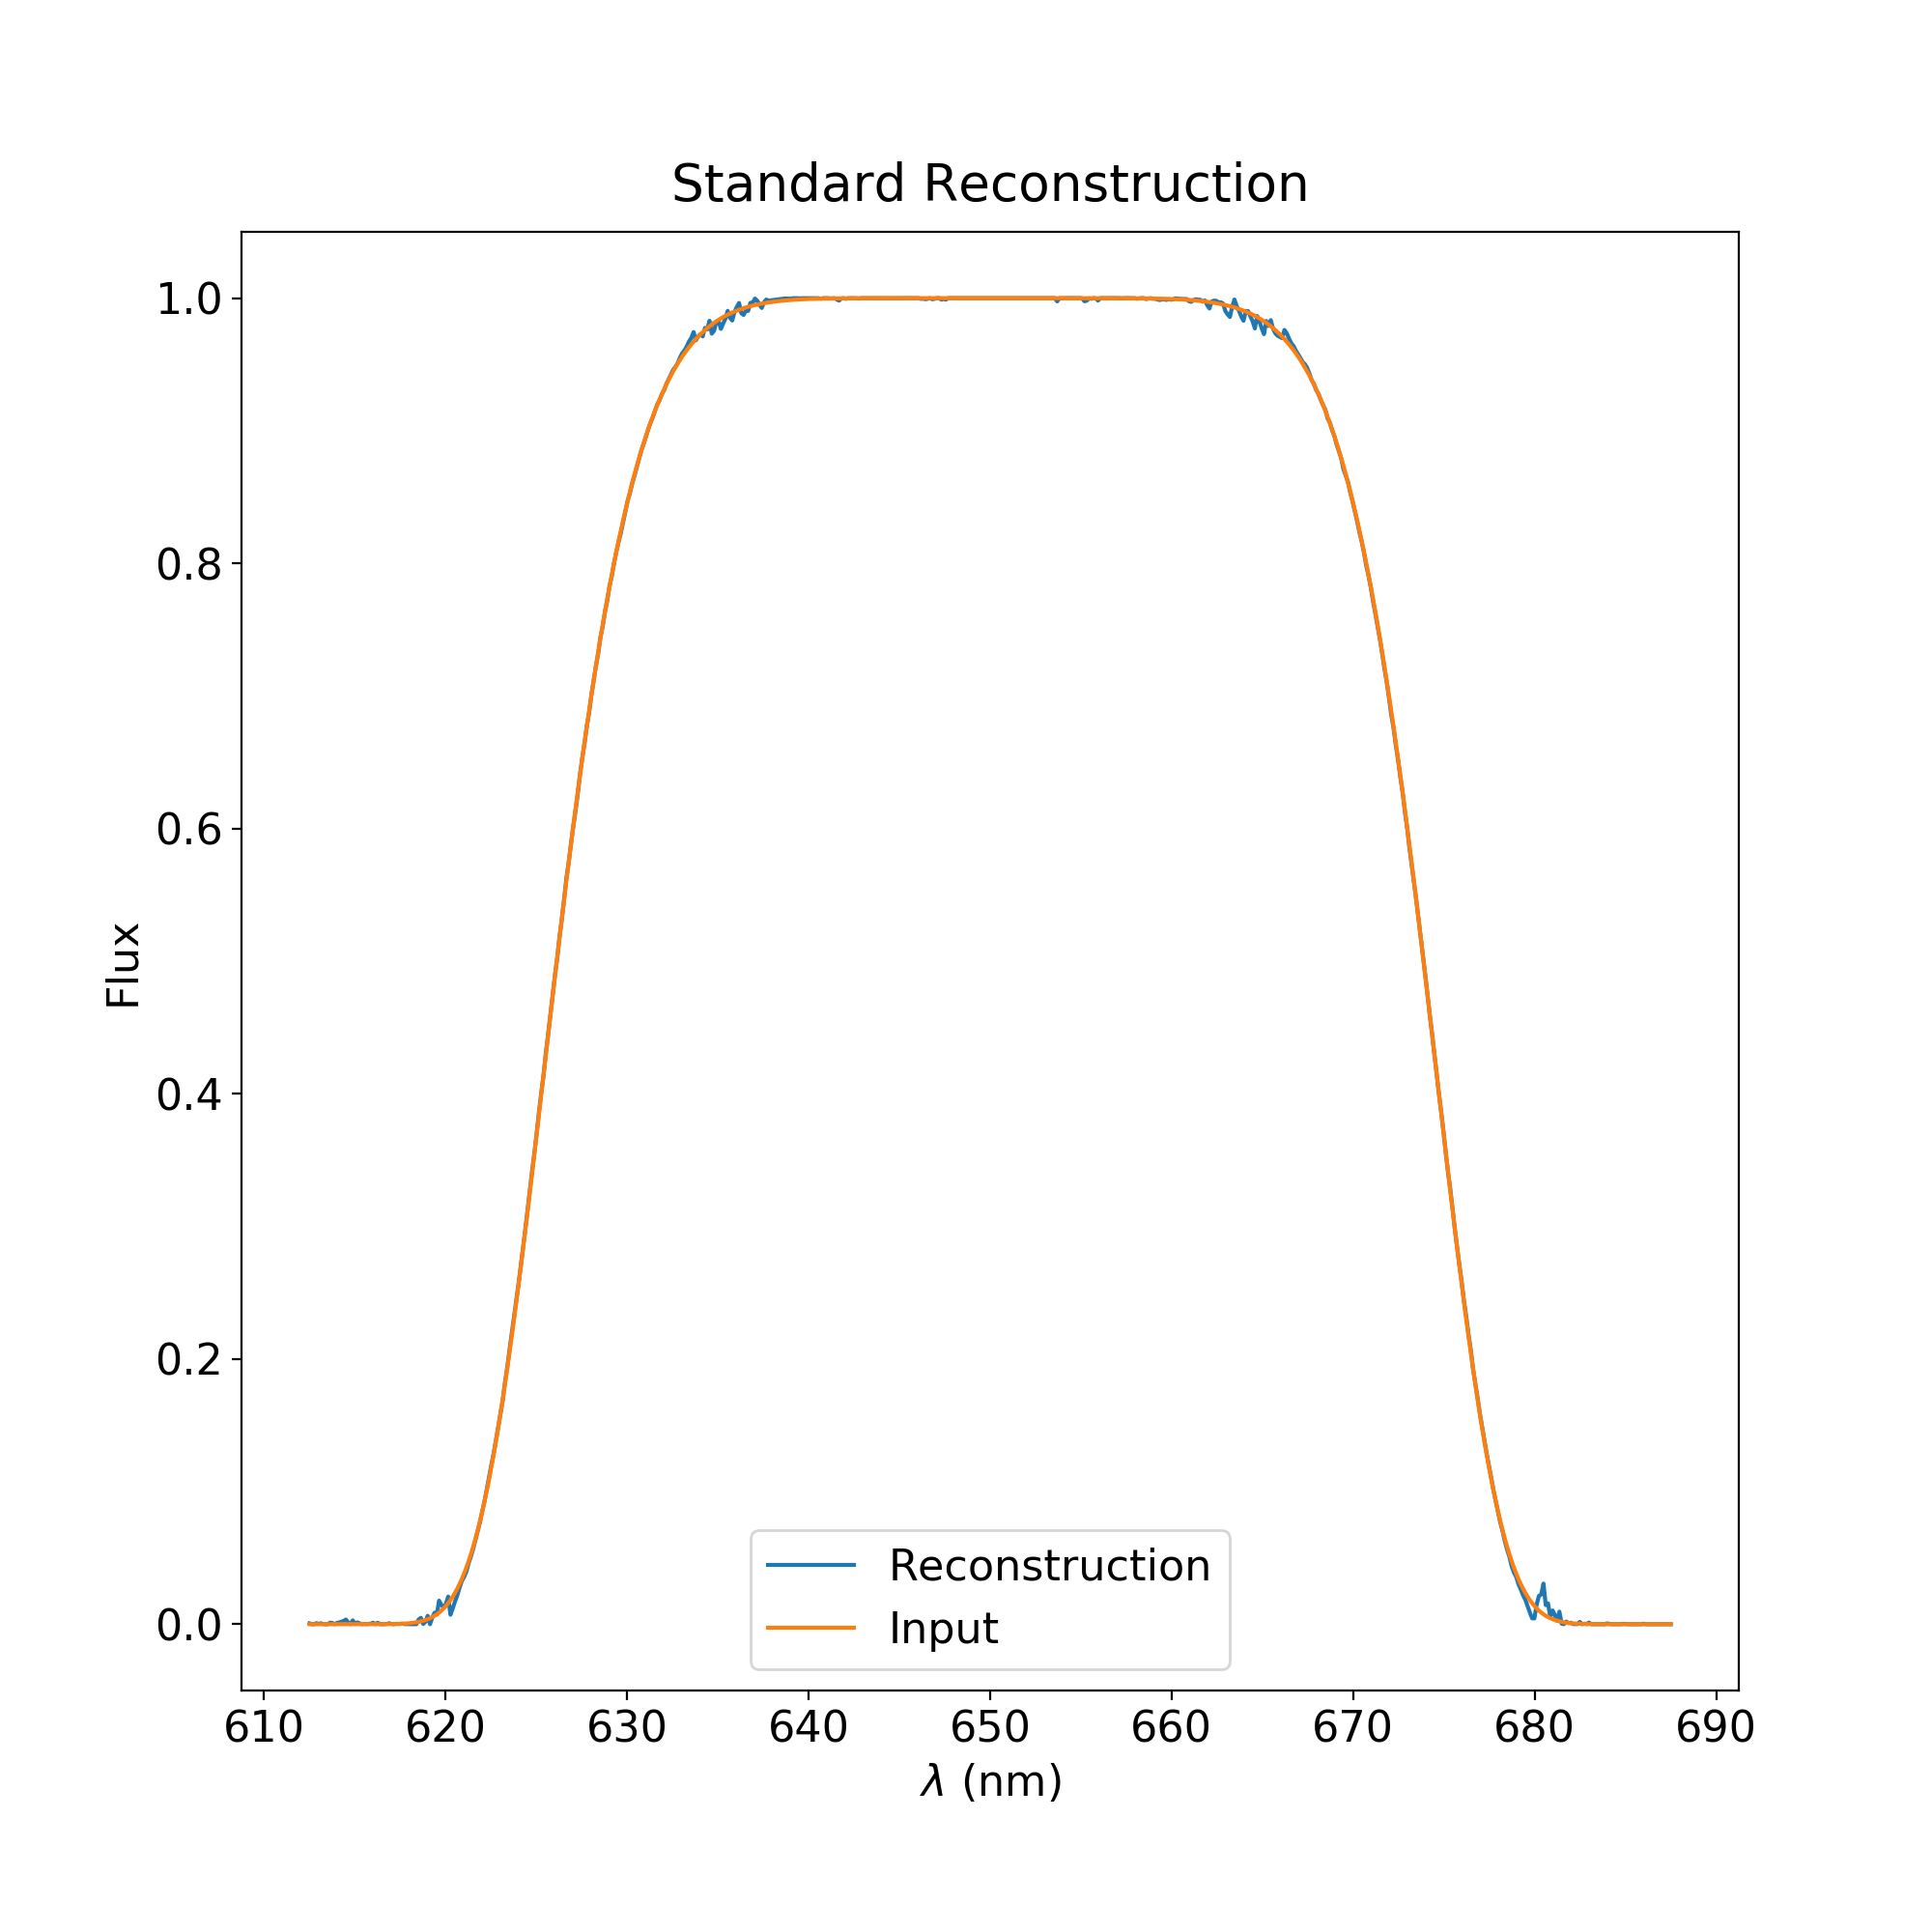
\includegraphics[width=0.75\textwidth]{standard_recon.png}
\caption{Orange: input spectrum. Blue: reconstruction with constrained least squares.}
\label{spectrum}
\end{figure}

\section{Further Questions}

To get some idea of the spectral response function, in Figure~\ref{response} I display the normalized dot product of the centre wavelength PSF with each other PSF in the ensemble. We see a sharp central feature with very strong sidelobes. Deconvolving these sidelobes out will be a major issue: will our funky diffractive pupil PSF make it too hard to extract a spectrum? Should we factor this into the design?

\begin{figure}
\centering
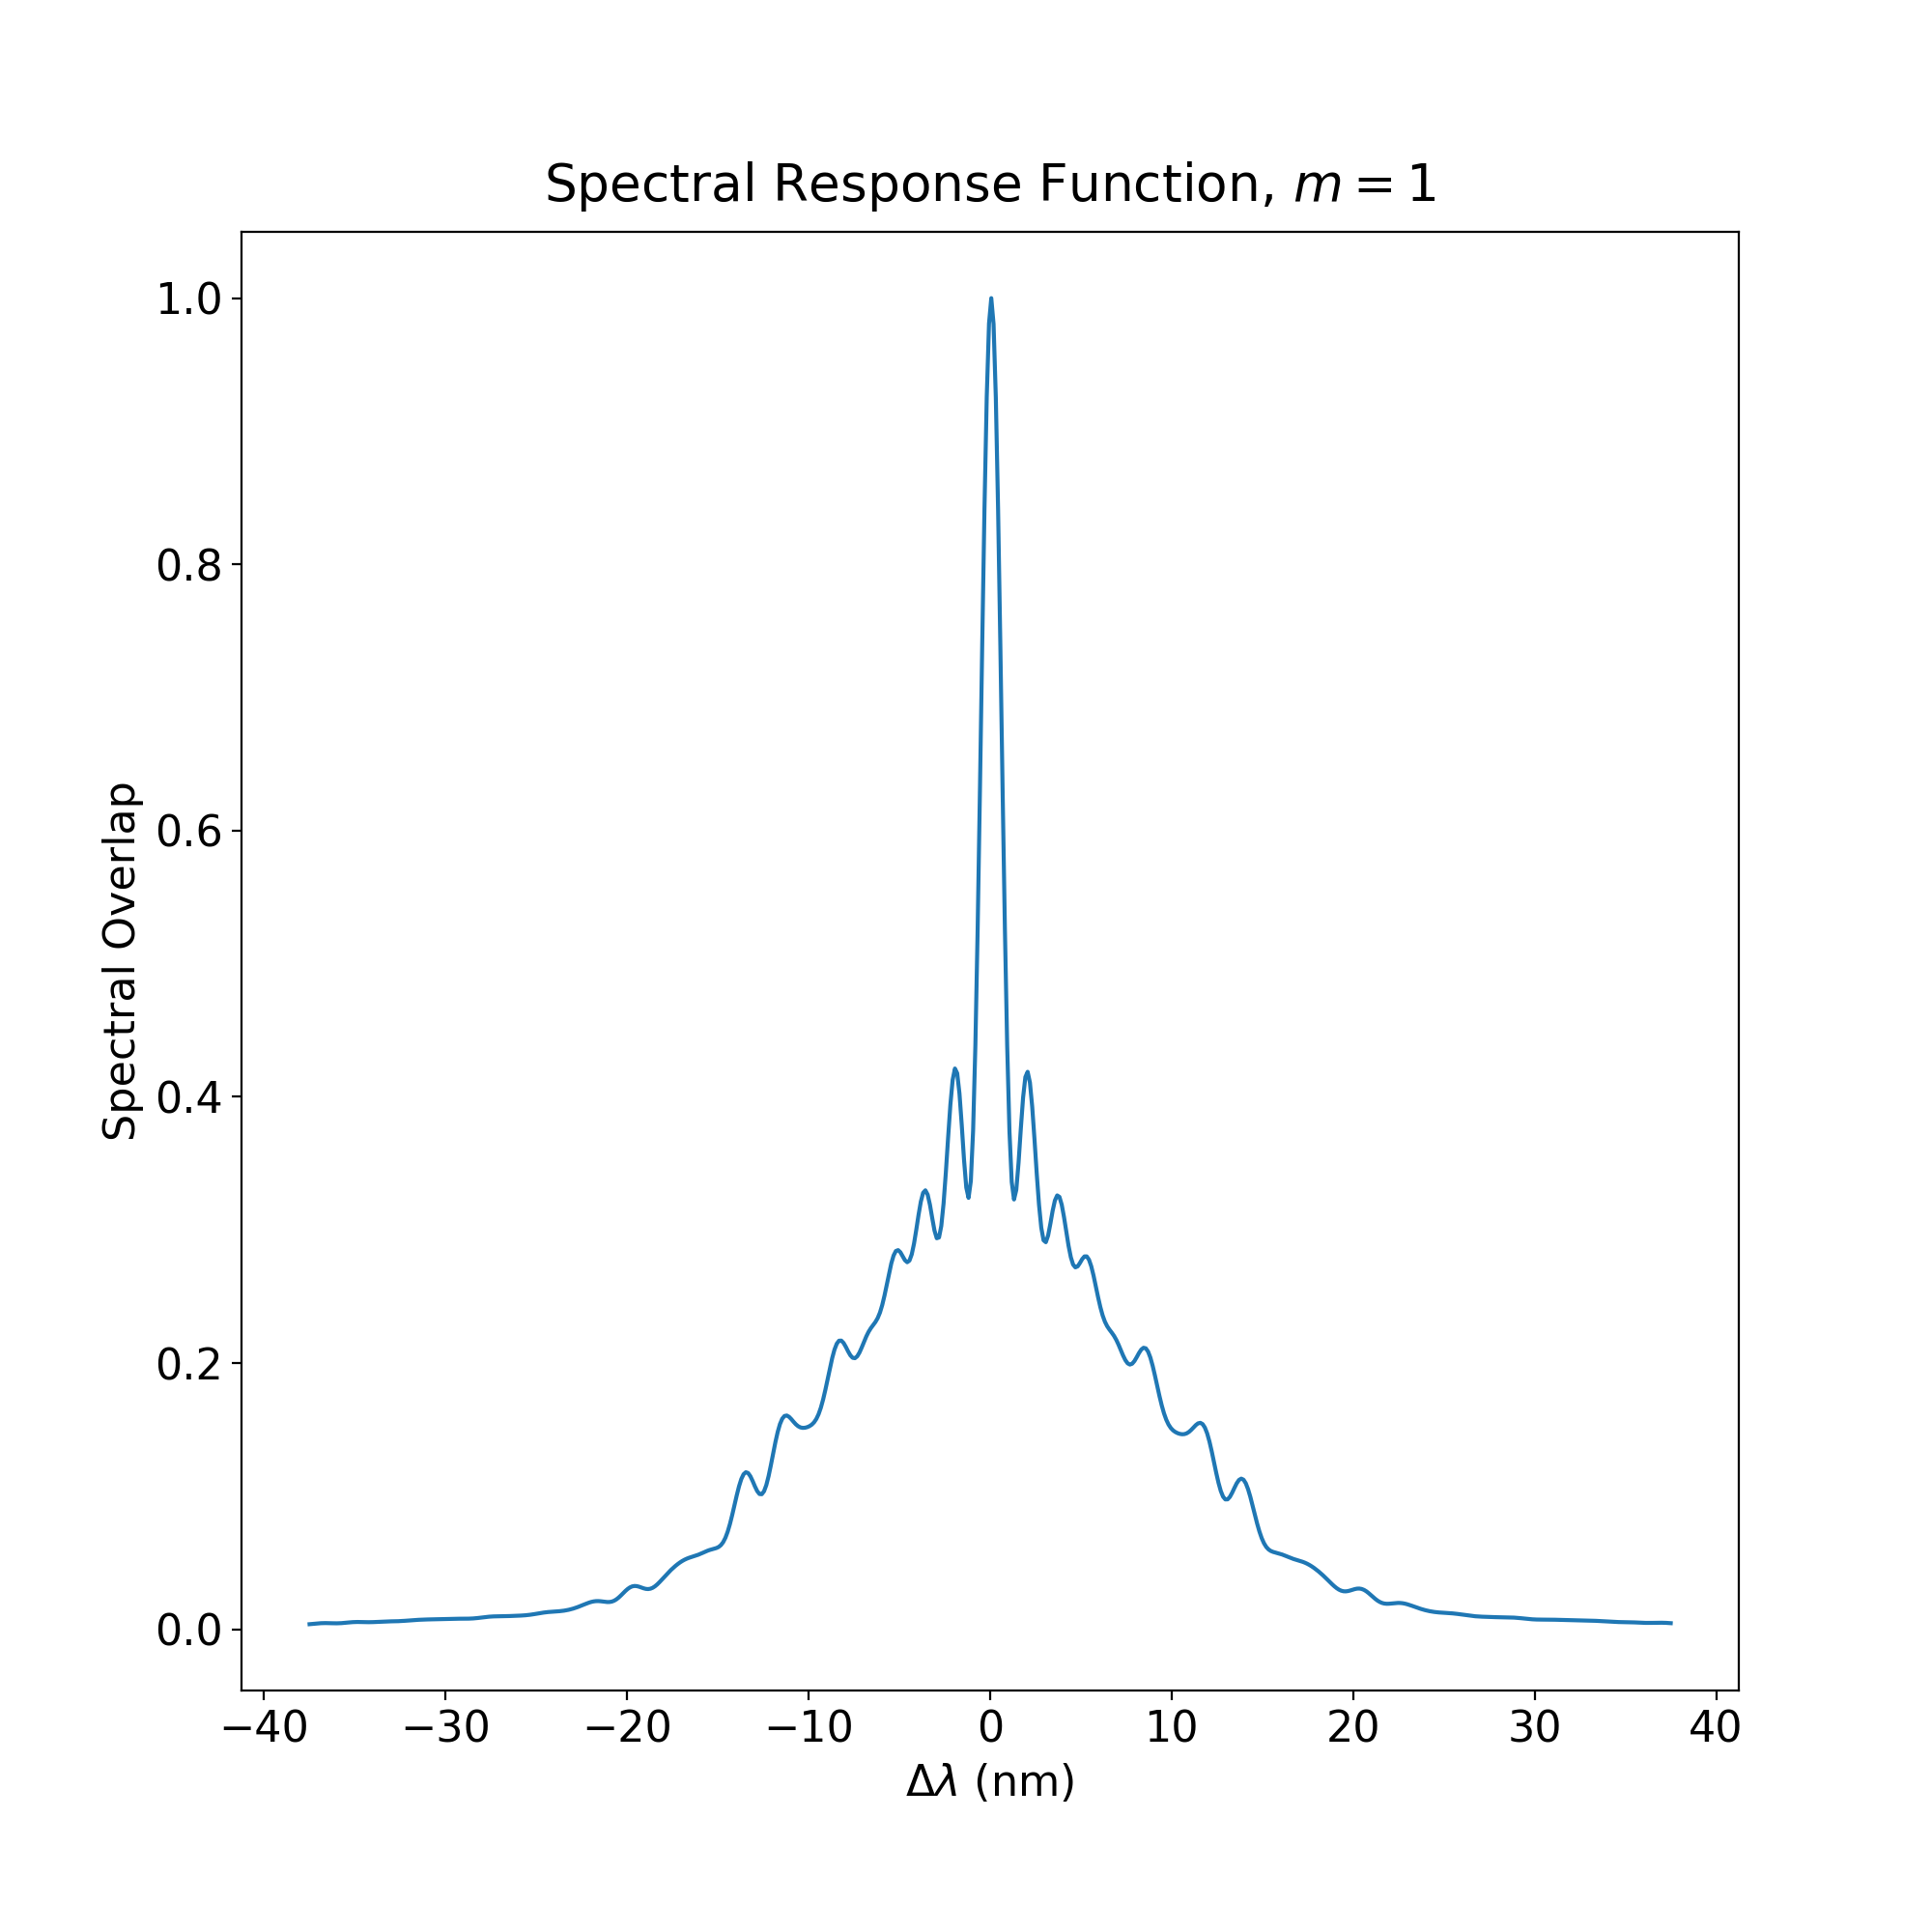
\includegraphics[width=0.75\textwidth]{specresponse.png}
\caption{Dot product of central PSF with other wavelengths. Note the strong sidelobes.}
\label{response}
\end{figure}

If we use an array of microdots to generate these diffraction patterns, we will also generate a lot of higher-order spots which will contribute to stray light. Peter has considered a phase mask of pure sine waves: is this achievable?

Can we use these first-order diffractive spots to help constrain the plate scale?

Will crosstalk between the spectra of $\alpha$~Cen~A and~B kill us?

\end{document}